% =============================================================================
%  VentCon: PID Control Demonstrator — User Manual
%  Target: max. 5 pages (excluding title page)
%  Document class: KOMA-Script scrartcl
% =============================================================================
\documentclass[
    11pt,
    a4paper,
    parskip=half-,          % half-line paragraph skip, no indent
    headings=normal,        % slightly smaller headings than default
    captions=tableheading,  % proper spacing for table captions
    numbers=noenddot        % no trailing dot after section numbers
]{scrartcl}

% --- Packages ----------------------------------------------------------------
\usepackage[utf8]{inputenc}
\usepackage[T1]{fontenc}
\usepackage{lmodern}                      % Latin Modern — clean, scalable
\usepackage{graphicx}
\usepackage[margin=2cm, top=2.4cm, bottom=2cm]{geometry}
\usepackage{hyperref}
\usepackage{xcolor}
\usepackage{booktabs}
\usepackage{enumitem}
\usepackage{scrlayer-scrpage}              % KOMA header/footer (replaces fancyhdr)
\usepackage[skins]{tcolorbox}               % coloured info boxes
\usepackage{float}
\usepackage{amsmath, amssymb, array}
\usepackage{caption}

% --- Colors ------------------------------------------------------------------
\definecolor{ventrexblue}{RGB}{0,47,135}
\definecolor{ventrexgreen}{RGB}{50,192,157}

% --- Hyperref ----------------------------------------------------------------
\hypersetup{
    colorlinks=true,
    linkcolor=ventrexblue,
    urlcolor=ventrexblue,
    hypertexnames=false
}

% --- KOMA fonts for headings -------------------------------------------------
\addtokomafont{disposition}{\color{ventrexblue}}   % all headings in brand colour
\addtokomafont{section}{\large}
\addtokomafont{subsection}{\normalsize}
\setkomafont{pagehead}{\small\normalfont\color{ventrexblue}}
\setkomafont{pagefoot}{\small\normalfont}

% --- Header / Footer (scrlayer-scrpage) --------------------------------------
\pagestyle{scrheadings}
\clearpairofpagestyles
\ihead{VentCon -- PID Control Demonstrator}
\ohead{User Manual v1.0}
\cfoot{\pagemark}
\KOMAoptions{headsepline=0.4pt}           % line below header

% --- Compact lists -----------------------------------------------------------
\setlist{nosep, leftmargin=1.5em}

% --- Smaller captions --------------------------------------------------------
\captionsetup{font=small, labelfont=bf, skip=4pt}

% =============================================================================
\begin{document}

% ========================== TITLE PAGE =======================================
\begin{titlepage}
    \pagenumbering{gobble}
    \centering
    \vspace*{1.5cm}

    
\includegraphics[width=0.75\textwidth]{pic/VENTREX_Logo + Slogan.pdf}

    \vspace{1.2cm}
    {\Huge\bfseries\textcolor{ventrexblue}{VentCon - PID Control Demonstrator}\par}
    \vspace{0.4cm}


    {\Huge User Manual\par}

    \vspace{2cm}
    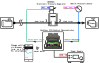
\includegraphics[width=0.90\textwidth]{pic/SchematicHardware.pdf}

    \vfill
    {\large Version 2.6\par}
    {\large \today\par}
\end{titlepage}

% ========================== BODY =============================================
\pagenumbering{arabic}

% ---------- SECTION 1: SYSTEM OVERVIEW ---------------------------------------
\section{System Overview}

Unlike a mechanical pressure regulator, which relies on a diaphragm and spring to maintain its setpoint,
the VENTREX electronic pressure regulator uses a software-based feedback control loop.
A PID algorithm continuously compares the measured outlet pressure with the desired setpoint and modulates the 
proportional valve accordingly.

The VentCon demonstrator showcases this principle: it implements the complete control loop on an ESP32-S3 
microcontroller, allowing users to observe and tune the regulator's behaviour in real time.
This document covers the system's hardware, functional principles, and browser-based user interface.


\begin{figure}[H]
    \centering
    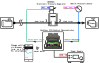
\includegraphics[width=1\textwidth]{pic/SchematicHardware.pdf}
    \caption{VentCon system overview.}
    \label{fig:overview}
\end{figure}

All parameters can be adjusted through a browser-based interface served over WiFi directly from the device---no external software, router, or internet connection is required.
The VentCon operates fully self-contained, making it usable in any environment regardless of existing network infrastructure.

\vfill

\begin{tcolorbox}[
    colback=ventrexblue!8,
    colframe=ventrexblue,
    fonttitle=\bfseries,
    title=Important,
    boxrule=0.6pt,
    arc=2pt
]
The PID control loop runs independently of the WiFi connection.
Even if the browser is closed or the device is disconnected from WiFi, pressure regulation continues uninterrupted 
based on the last applied settings---as long as the power supply remains on. \\[1ex]
This also means that upon switching the power supply on, the system will immediately start to regulate the pressure.
\end{tcolorbox}

\pagebreak


% ---------- SECTION 2: GETTING STARTED --------------------------------------
\section{Getting Started}

\subsection{Wiring Scheme}

The terminal block on the front of the unit (Figure~\ref{fig:terminal}) provides connections for the proportional valve 
(\texttt{PV+}/\texttt{PV-}), the pressure sensor (\texttt{Sen}/\texttt{Sup}/\texttt{GND}), and the power supply 
(\texttt{VIn}/\texttt{GND}).

The connector for the PV is included in the demo kit, thus the user only needs to connect the pressure sensor and the power supply.
The pressure sensor (not included in the demo kit) requires three connections: \texttt{Sup} provides regulated 5\,V 
supply for the sensor, while \texttt{GND} serves as the sensor's ground reference. The \texttt{Sen} terminal is the input for the 
sensor's pressure signal, which the controller uses to regulate the outlet pressure.

The power supply (not included) should provide a stable DC voltage. For the PV delivered in this demo kit, 
the recommended voltage is 12\,V (connected to \texttt{VIn})\footnote{the device can operate with any supply voltage in the range of 12 to 
30\,V}, while the \texttt{GND}\footnote{The \texttt{GND} terminal serves as the common ground reference for the entire system} 
is connected to the negative terminal of the power supply.

\begin{figure}[H]
    \centering
        \centering
        \includegraphics[width=0.9\linewidth]{pic/Terminal_block.pdf}
        \caption{Terminal block connections.}
        \label{fig:terminal}
\end{figure}


\subsection{Connecting to the Device}



\begin{figure}[H]
    \centering

        \centering
        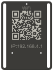
\includegraphics[width=0.5\linewidth]{pic/BackSide.pdf}
        \caption{Rear view of the VentCon unit.}
        \label{fig:backside}

\end{figure}

The VentCon creates its own WiFi access point---no router or internet connection is needed.

\begin{enumerate}
    \item \textbf{Power on} the VentCon unit.
    \item On your smartphone, tablet or PC, open \textbf{WiFi settings}.
    \item Connect to the network \texttt{VENTCON\_AP}.
    \item Enter the password: \texttt{ventcon12!}
    \item Open a web browser and navigate to \textbf{\url{http://192.168.4.1}}\\
          (alternatively \textbf{\url{http://ventcon.local}}).
\end{enumerate}

\begin{table}[H]
\centering\small
\begin{tabular}{@{}ll@{}}
\toprule
\textbf{Setting}        & \textbf{Default Value} \\
\midrule
Network Name (SSID)      & \texttt{VENTCON\_AP} \\
Password                 & \texttt{ventcon12!} \\
IP Address               & \texttt{192.168.4.1} \\
Max.\ simultaneous clients & 2 \\
\bottomrule
\end{tabular}
\caption{WiFi connection details.}
\end{table}

\noindent\textit{Note:} The PID control loop runs independently of the WiFi connection.
Disconnecting the browser does \emph{not} stop pressure regulation.

\subsection{Browser Compatibility}

The web interface works with all modern browsers, e.g. Google Chrome or Safari.


\subsection{Functional Principle}

Figure~\ref{fig:pid-block} illustrates the closed-loop control architecture.
A pressure sensor continuously measures the outlet pressure (\emph{Process Variable}).
The PID controller computes the error between the \emph{Setpoint} and the measured pressure, and outputs a \emph{Valve Duty Cycle} (PWM signal) to the solenoid valve.

\begin{figure}[H]
    \centering
    \includegraphics[width=\linewidth]{pic/PID_blockDiagram.pdf}
    \caption{PID closed-loop control block diagram.
             The Setpoint is compared with the Outlet Pressure; the error drives
             the Proportional, Integral and Derivative paths whose sum controls
             the Valve Duty Cycle.}
    \label{fig:pid-block}
\end{figure}




% ---------- SECTION 3: WEB INTERFACE ----------------------------------------
\section{Web Interface}

The web interface is divided into collapsible sections (tap a header to expand/collapse).
Figure~\ref{fig:browser-app} provides an annotated overview.

\begin{figure}[H]
    \centering
    \includegraphics[width=\linewidth]{pic/BrowserApp.pdf}
    \caption{Annotated overview of the VentCon browser application.}
    \label{fig:browser-app}
\end{figure}

\subsection{Real-Time Monitoring}

\begin{itemize}
    \item \textbf{Outlet Pressure} gauge---current pressure in bar(g) with a target marker at the setpoint and a trend indicator ($\blacktriangle$\,rising / $\blacktriangledown$\,falling / $=$\,stable).
    \item \textbf{Valve Duty Cycle} gauge---current PID output as a percentage (0--100\,\%).
    \item \textbf{Live Chart}---time-series plot of:
        \begin{itemize}
            \item \textcolor{blue}{Blue line}: Outlet Pressure (Process Variable)
            \item \textcolor{orange}{Orange dashed line}: Setpoint
            \item \textcolor{green!60!black}{Green line}: Valve Duty Cycle
        \end{itemize}
    Toggle the chart with the \emph{Show Chart} checkbox. Disabling it can improve performance on slower devices.
\end{itemize}

\subsection{Control Parameters}

\begin{itemize}
    \item \textbf{Setpoint Outlet Pressure}---target pressure in bar(g). Adjusted via slider, $+$/$-$ buttons, or direct numerical input.
    \item \textbf{Kp, Ki, Kd}---PID gains (see Section~\ref{sec:pid}).
    \item \textbf{Reset PID} button---clears the controller's internal state (integral sum and derivative history).
\end{itemize}

Each slider's range can be customised by tapping the gear icon next to the slider label.

\subsection{Auxiliary Settings}

\begin{itemize}
    \item \textbf{Low Pass Filter ($\alpha$)}---filter strength applied to the pressure sensor signal (0\,=\,off, 1\,=\,maximum smoothing).
    \item \textbf{Actuator PWM Frequency}---solenoid drive frequency (100--10\,000\,Hz).
    \item \textbf{Actuator PWM Resolution}---duty-cycle resolution (8--16\,bit).
    \item \textbf{PID Sample Time}---control loop period in ms.
\end{itemize}

\subsection{Applying Changes}

Changes are \textbf{not} applied immediately.
After adjusting any parameter a blue \textbf{Apply Changes} button appears at the bottom of the screen (Figure~\ref{fig:apply}).
Tap it to send all pending changes to the device.
All applied settings are automatically persisted to flash memory and survive power cycles.

\begin{figure}[H]
    \centering
    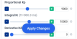
\includegraphics[width=0.55\textwidth]{pic/ApplyButton.pdf}
    \caption{The floating \emph{Apply Changes} button appears when parameters have been modified.}
    \label{fig:apply}
\end{figure}

% ---------- SECTION 4: PID CONTROL BASICS -----------------------------------
\section{PID Control Basics}\label{sec:pid}

The VentCon uses the \emph{Parallel Form} (non-interacting form) of the PID algorithm.
Each control action is computed independently and summed:

\begin{equation}
y(t) \;=\; K_p \, e(t) \;+\; K_i \!\int_0^t e(\tau) \, d\tau \;+\; K_d \, \frac{de(t)}{dt}
\label{eq:pid}
\end{equation}

\noindent where $y(t)$ is the controller output (Valve Duty Cycle), $e(t)$ is the error (Setpoint\,$-$\,Outlet Pressure), and $K_p$, $K_i$, $K_d$ are the tunable gains.

\begin{table}[H]
\centering\small
\begin{tabular}{c|l|l}
\textbf{Term} & \textbf{Role} & \textbf{Focus} \\ \hline
$K_p$ (Proportional) & Present & Reacts to \emph{how far} you are from target \\
$K_i$ (Integral)     & Past    & Reacts to \emph{how long} you have been away \\
$K_d$ (Derivative)   & Future  & Reacts to \emph{how fast} you are approaching/leaving
\end{tabular}
\caption{PID term summary.}
\end{table}

\paragraph{Proportional ($K_p$).}
Output proportional to the current error.
Higher $K_p$ gives a more aggressive response but can cause overshoot.

\paragraph{Integral ($K_i$).}
Accumulates past error to eliminate steady-state offset.
Too high a value causes oscillation (integral windup).

\paragraph{Derivative ($K_d$).}
Damps the response by reacting to the rate of change of the error.
Reduces overshoot but amplifies sensor noise if set too high.

% ---------- SECTION 5: TUNING GUIDE -----------------------------------------
\section{Tuning Guide}

Follow these steps for initial tuning. Observe the \textbf{Live Chart} after each change.

\begin{enumerate}
    \item \textbf{Set a Stable Operating Point.}
          Choose a moderate setpoint (e.g.\ 4.00\,bar) and let the system settle.

    \item \textbf{Start with P-only control.}
          Set $K_i = 0$ and $K_d = 0$.
          Begin with a low $K_p$ and increase gradually.
          Find the value where the pressure just begins to oscillate steadily (\emph{ultimate gain}), then back off slightly.

    \item \textbf{Introduce Integral action.}
          Slowly increase $K_i$ to remove the remaining steady-state offset.
          Stop increasing when further gains cause oscillation.

    \item \textbf{Add Derivative action (if needed).}
          If the response overshoots or is slow to settle, increase $K_d$ cautiously to add damping.

    \item \textbf{Iterate.}
          Make small single-parameter changes and observe.
          The goal is a fast, smooth response with minimal overshoot.
\end{enumerate}

\subsection{Example: Step Response}

Figure~\ref{fig:step} shows a typical step-response recording where the setpoint is changed from 4 to 6\,bar.
Figure~\ref{fig:disturbance} demonstrates the controller rejecting a mass-flow disturbance while maintaining the setpoint.

\begin{figure}[H]
    \centering
    \begin{minipage}[t]{0.48\textwidth}
        \centering
        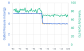
\includegraphics[width=\linewidth]{pic/Example_Set_4_to_6_bar.pdf}
        \caption{Setpoint step from 4 to 6\,bar.}
        \label{fig:step}
    \end{minipage}\hfill
    \begin{minipage}[t]{0.48\textwidth}
        \centering
        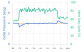
\includegraphics[width=\linewidth]{pic/Example_Regulator_Action_Massflow_Variation.pdf}
        \caption{Disturbance rejection under varying mass flow.}
        \label{fig:disturbance}
    \end{minipage}
\end{figure}

% ---------- SECTION 6: QUICK REFERENCE --------------------------------------
\section{Quick Reference}

\begin{table}[H]
\centering\small
\begin{tabular}{@{}ll@{}}
\toprule
\textbf{Action}              & \textbf{How To} \\
\midrule
Connect to device             & WiFi: \texttt{VENTCON\_AP} / Password: \texttt{ventcon12!} \\
Open web interface            & Browser $\rightarrow$ \texttt{http://192.168.4.1} \\
Expand / collapse sections    & Tap section header \\
Adjust setpoint               & Drag slider or use $+$/$-$ buttons \\
Fine-tune PID                 & Adjust $K_p$, $K_i$, $K_d$ sliders \\
Customise slider range        & Tap gear icon next to slider label \\
Apply changes                 & Tap blue \emph{Apply Changes} button \\
Reset PID state               & Tap \emph{Reset PID} button \\
Toggle live chart             & Use \emph{Show Chart} checkbox \\
Reset to factory defaults     & Use \emph{Reset to Default} in System Info \\
\bottomrule
\end{tabular}
\caption{Quick reference card.}
\end{table}

\end{document}